\documentclass[11pt,letterpaper]{article}
\usepackage[T1]{fontenc}
\usepackage[utf8]{inputenc}
\usepackage{lmodern}
\usepackage[margin=0.85in]{geometry}
\usepackage{amsmath,amssymb,booktabs,tabularx}
\usepackage{xcolor}
\usepackage{tikz}
\usetikzlibrary{arrows.meta,positioning,calc}
\usepackage{listings}
\usepackage{xurl}
\usepackage{hyperref}
\usepackage{microtype}
\usepackage{needspace}
\definecolor{accent}{HTML}{185A78}
\definecolor{pale}{HTML}{EDF5F8}
\hypersetup{colorlinks=true,linkcolor=accent,urlcolor=accent}
\lstset{basicstyle=\ttfamily\small,breaklines=true,columns=fullflexible,
  keepspaces=true,showstringspaces=false,backgroundcolor=\color{pale},
  frame=single,rulecolor=\color{accent!25},xleftmargin=5pt,xrightmargin=5pt}
\tikzset{box/.style={draw=accent,fill=pale,rounded corners=3pt,
  align=center,minimum height=11mm,font=\small},
  flow/.style={-{Stealth[length=2mm]},thick,draw=accent}}
\setlength{\parindent}{0pt}
\setlength{\parskip}{6pt}
\setlength{\emergencystretch}{2em}
\title{\textbf{FSCK-NN}\\[0.4em]\large Reference-temperature theory, database format, and PyTorch training}
\author{Project implementation guide}
\date{\small Based on the current FSCK-NN source code}
\begin{document}
\maketitle
\vspace{-1em}
This guide describes the existing 32-point FSK V4 database and the
\textbf{kappa-only} training pipeline. The network has seven physical inputs
and 32 kappa outputs. No a-function targets or intermediate CSV files are used.
The final section explains why reference temperature remains an input.

\section{FSCK Database file names and format}
\subsection{Directory and filename convention}
The default database directory is
\begin{lstlisting}
<your path>/FSKTableV4
\end{lstlisting}
This default is defined by \texttt{DEFAULT\_DB} in
\path{training/fsck_backend.py}. You can also specify the path in the training script \path{training/train_fsck.py} using command-line argument \texttt{--database}. From the \texttt{FSCK\_NN} directory, run:
\begin{lstlisting}[language=bash]
python3 training/train_fsck.py --database /path/to/FSKTableV4
\end{lstlisting}

Each pressure has a subdirectory, such as \texttt{01.0} for 1 atm.
One file identifies a fixed pressure and composition. For example:
\begin{lstlisting}
01.0/P.01.0_CO2.0.00_H2O.0.00_CO.0.00_fv.1.E-05_k.dat
\end{lstlisting}
The general pattern is
\begin{lstlisting}
P.<P>_CO2.<xCO2>_H2O.<xH2O>_CO.<xCO>_fv.<fv>_k.dat
\end{lstlisting}
\begin{center}
\begin{tabularx}{\linewidth}{@{}l X@{}}
\toprule
Token & Meaning and database range \\
\midrule
\texttt{P} & Pressure in atmospheres, $0.1$--$80$ atm.
34 grid values: 0.1, 0.2, 0.3, 0.4, 0.5, 0.7, 1, 2, 3, 4, 5, 6, 7,
8, 9, 10, 11, 12, 13, 14, 15, 20, 25, 30, 35, 40, 45, 50, 55, 60,
65, 70, 75, 80. \\
\addlinespace
\texttt{CO2} & Carbon dioxide mole fraction, $0$--$1$.
10 grid values: 0, 0.01, 0.02, 0.03, 0.04, 0.05, 0.25, 0.5, 0.75, 1. \\
\addlinespace
\texttt{H2O} & Water vapor mole fraction, $0$--$1$.
13 grid values: 0, 0.01, 0.02, 0.03, 0.04, 0.05, 0.1, 0.15, 0.2, 0.25,
0.5, 0.75, 1. \\
\addlinespace
\texttt{CO} & Carbon monoxide mole fraction, $0$--$0.5$.
6 grid values: 0, 0.01, 0.05, 0.1, 0.25, 0.5. \\
\addlinespace
\texttt{fv} & Dimensionless soot volume fraction,
$0$--$10^{-5}$ (0--10 ppm by volume).
4 grid values: $0$, $10^{-7}$, $10^{-6}$, $10^{-5}$. \\
\addlinespace
\texttt{\_k.dat} & Binary kappa table \\
\bottomrule
\end{tabularx}
\end{center}
The prefix separator and decimal point are distinct: \texttt{P.01.0}
contains the prefix \texttt{P.} followed by the number \texttt{01.0}.
The Python reader parses these values from the filename and checks that the
pressure agrees with its directory.

The pressure and composition ranges and grid values in the table come from
\texttt{PDB}, \texttt{xCO2DB}, \texttt{xH2ODB}, \texttt{xCODB}, and \texttt{fvDB} in
\texttt{fskTableV4.f90}. They describe the full declared database axes;
\texttt{loadIntoMem} may load a subset according to the requested limits and
available files. The listed gas mole fractions must sum to at most unity
for a physical mixture.

\subsection{Temperature dimensions and record ordering}
Each file contains every pair of local gas temperature $T_g$ and reference
Planck-weighting temperature $T_r$ on the grid
\[
T_i=300+100(i-1)\ \mathrm{K},\qquad i=1,\ldots,28.
\]
Therefore there are $28\times28=784$ binary records per file. The reference
temperature varies fastest. With one-based indices,
\[
\boxed{r=28(i_g-1)+i_r},\qquad 1\leq r\leq784.
\]
The reference temperature remains an NN input because the cumulative
Planck-weighted k-distribution depends on it, even when no a-function is trained.

\begin{figure}[htbp]
\centering
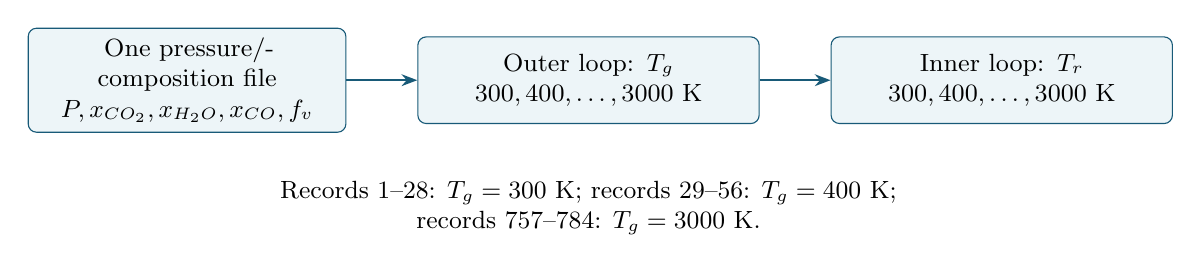
\begin{tikzpicture}[node distance=5mm]
\node[box,text width=38mm] (state) {One pressure/composition file\\$P,x_{CO_2},x_{H_2O},x_{CO},f_v$};
\node[box,right=9mm of state,text width=41mm] (local) {Outer loop: $T_g$\\$300,400,\ldots,3000$ K};
\node[box,right=9mm of local,text width=41mm] (ref) {Inner loop: $T_r$\\$300,400,\ldots,3000$ K};
\draw[flow] (state)--(local);
\draw[flow] (local)--(ref);
\node[below=6mm of local,align=center,font=\small] {Records 1--28: $T_g=300$ K; records 29--56: $T_g=400$ K;\nobreak\\records 757--784: $T_g=3000$ K.};
\end{tikzpicture}
\caption{Temperature-pair ordering within each database file.}
\end{figure}

\subsection{Binary record layout}
The existing reader uses Fortran unformatted \emph{direct-access} records.
There is no text header and no sequential-unformatted record marker. Each
record contains 33 single-precision floating-point values:
\[
[\kappa_1,\ldots,\kappa_{32},\kappa_{\max}].
\]
The first 32 values correspond to fixed quadrature nodes. The last is the
maximum-kappa value, not an additional quadrature point.
\begin{figure}[htbp]
\centering
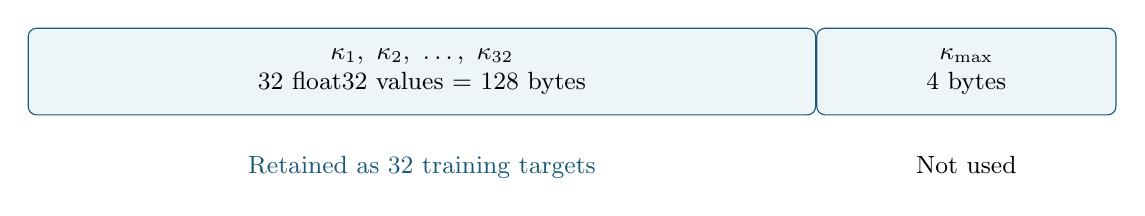
\begin{tikzpicture}
\node[box,minimum width=100mm] (k) {$\kappa_1,\ \kappa_2,\ \ldots,\ \kappa_{32}$\\32 float32 values = 128 bytes};
\node[box,right=0mm of k,minimum width=38mm] (max) {$\kappa_{\max}$\\4 bytes};
\node[below=4mm of k,font=\small,text=accent] {Retained as 32 training targets};
\node[below=4mm of max,font=\small] {Not used};
\end{tikzpicture}
\caption{One 132-byte record; byte offset of record $r$ is $132(r-1)$.}
\end{figure}
The expected file size is
\[
784\times33\times4=\boxed{103{,}488\ \text{bytes}}.
\]

In short each set of $(P,x_{CO_2},x_{H_2O},x_{CO},f_v,T_g,T_r)$ will give 32 $\kappa$ values to train with (excluding the $\kappa_{max}$).




\section{Train using the FSCK database}
\subsection{Project layout and requirements}
\begin{lstlisting}
FSCK_NN/
  fortran/                 # preserved numerical sources and row_bridge.inc
  training/
    train_fsck.py          # PyTorch model, batches, training, checkpoints
    fsck_backend.py        # binary reader and Fortran build/ctypes bridge
    pressure_selection.py  # pressure folder selection
    requirements.txt       # PyTorch and ONNX dependencies
    build/                 # generated Fortran module and shared library
    runs/                  # training output directories
  test/
    compare_fsck.f90       # NN / direct-database comparison
    FSCK_to_csv.f90        # standalone binary database CSV export
    build_FSCK_to_csv.sh   # build the CSV exporter without ONNX
    nn_model.f90           # Fortran ONNX interface
    onnx_bridge.c          # ONNX Runtime C API bridge
    comparison_grid.f90   # read the Fortran grid namelist
    grid.nml               # pressure/composition/temperature grid
    build.sh               # compile with external ONNX Runtime SDK
    plot_results.py        # plot the completed comparison CSV
    requirements.txt       # NumPy and Matplotlib for plotting
  docs/
    fsck_nn_guide.tex       # this document
\end{lstlisting}
Requirements are Python 3.9 or later, gfortran, PyTorch, and ONNX. The current build flags target gfortran;
Intel Fortran is not configured by these scripts. If the Python packages are not installed already, then
from the \texttt{FSCK\_NN} directory, install the Python dependencies:
\begin{lstlisting}[language=bash]
python3 -m pip install -r training/requirements.txt
\end{lstlisting}
A working Fortran compiler must be on \texttt{PATH}, or supplied using
\texttt{--compiler}. OpenFOAM is not needed to run this training program.

\subsection{Direct database-to-PyTorch workflow}
\begin{figure}[htbp]
\centering
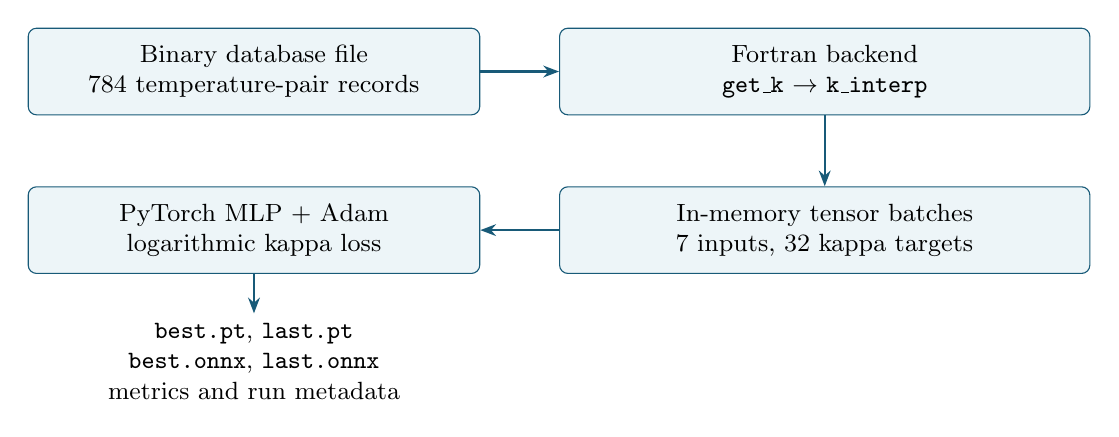
\begin{tikzpicture}[node distance=5mm]
\node[box,text width=55mm] (db) {Binary database file\\784 temperature-pair records};
\node[box,right=10mm of db,text width=65mm] (f) {Fortran backend\\\texttt{get\_k} $\rightarrow$ \texttt{k\_interp}};
\node[box,below=9mm of f,text width=65mm] (batch) {In-memory tensor batches\\7 inputs, 32 kappa targets};
\node[box,left=10mm of batch,text width=55mm] (nn) {PyTorch MLP + Adam\\logarithmic kappa loss};
\draw[flow] (db)--(f);
\draw[flow] (f)--(batch);
\draw[flow] (batch)--(nn);
\node[below=5mm of nn,align=center,font=\small] (out) {\texttt{best.pt}, \texttt{last.pt}\\\texttt{best.onnx}, \texttt{last.onnx}\\metrics and run metadata};
\draw[flow] (nn)--(out);
\end{tikzpicture}
\caption{Training uses database records directly; no CSV dataset is created.}
\end{figure}
The build injects \texttt{row\_bridge.inc} into a generated copy of the V4
module. A shared library is loaded through Python \texttt{ctypes}. For each
file, the bridge loads all temperature pairs into singleton pressure and
composition axes, then follows the kappa-only path of \texttt{fsk\_v4\_table}.
It does not calculate \texttt{afun}. Computed kappa values are checked against
the first 32 stored values at each grid record.

\subsection{Inputs, network, and loss}
The physical input vector is
\[
\mathbf{x}=(P_{\mathrm{atm}},x_{CO_2},x_{H_2O},x_{CO},f_v,T_g,T_r),
\]
and the target vector is $(\kappa_1,\ldots,\kappa_{32})$.
The default MLP has three hidden layers of 128 units with SiLU activations.
Input preprocessing is part of the model:
\begin{align*}
P'&=\frac{\log_{10}P+1}{\log_{10}800}, &
f_v'&=\frac{\ln(1+f_v/10^{-9})}{\ln(1+10^{-5}/10^{-9})},\\
T_g'&=\frac{T_g-300}{2700}, & T_r'&=\frac{T_r-300}{2700}.
\end{align*}
Mole fractions are unchanged. These scales are fixed and do not use validation
statistics. Input values are not clipped to these nominal ranges.

The network predicts $z_i=\log_{10}\kappa_i$. Training minimizes
\[
\mathcal{L}=\frac{1}{32B}\sum_{b=1}^{B}\sum_{i=1}^{32}
\left[z_{b,i}-\log_{10}\!\left(\max(\kappa_{b,i},\kappa_{\mathrm{floor}})\right)\right]^2,
\qquad \kappa_{\mathrm{floor}}=10^{-8}.
\]
The floor is in native database units and handles zero kappas. Values below it
are not distinguished by the loss. \texttt{forward()} returns logarithmic
predictions, while \texttt{predict\_kappa()} returns $10^{z_i}$. No constraint
forces predictions to be monotonic across quadrature nodes.

\subsection{Training commands}
All commands below run from the \texttt{FSCK\_NN} directory. Start with a small pipeline
check; the first six sorted files are not a representative training dataset.
\begin{lstlisting}[language=bash]
python3 training/train_fsck.py \
  --pressure 1 --limit-files 6 --epochs 2 \
  --output training/runs/my_smoke
\end{lstlisting}
Train using all files at 1 atm:
\begin{lstlisting}[language=bash]
python3 training/train_fsck.py \
  --pressure 1 --epochs 20 \
  --output training/runs/one_atm
\end{lstlisting}
Train using every pressure and composition:
\begin{lstlisting}[language=bash]
python3 training/train_fsck.py \
  --pressures all --epochs 20 \
  --output training/runs/full_database
\end{lstlisting}
Select existing pressure folders with \texttt{--pressures}. Values are in atm;
\texttt{01.0} and \texttt{1} select the same pressure. Use \texttt{all} (the
default), a single value, an inclusive range \texttt{low:high}, or a
comma-separated list. Values and ranges may be combined:
\begin{lstlisting}[language=bash]
python3 training/train_fsck.py --pressures 1:5
python3 training/train_fsck.py --pressures 0.5,1,3
python3 training/train_fsck.py --pressures 0.5,2:5
\end{lstlisting}
Ranges select existing folders, not a generated pressure grid. For example,
\texttt{1.5:3} includes 2 and 3 atm folders if present. Duplicate selections
are included once. Each requested value or range must match at least one
folder. Invalid numbers, reversed ranges, and unmatched selections produce
errors. The original \texttt{--pressure 1} option remains an alias.
Actual folders used are printed and recorded in \texttt{run.json}.
The \texttt{--limit-files} cap is applied after filtering across all selected
pressures, so a small cap can include only the lowest selected pressure.

Use a new or empty output directory for each run. To use another database,
add \texttt{--database} followed by the database path. Without \texttt{--output}, a
timestamped folder is created under \path{training/runs}.

\begin{center}
\begin{tabularx}{\linewidth}{@{}l l X@{}}
\toprule
Option & Default & Purpose \\
\midrule
\texttt{--database} & \texttt{DEFAULT\_DB} & Database root directory; defaults to
\path{/Volumes/home/cnp10/CODES/radiationDatabase/FSKTableV4}, defined in
\texttt{fsck\_backend.py} \\
\texttt{--limit-files} & No limit & First $N$ sorted files after pressure filtering,
shared across training and validation. For example, 6 files give 4,704 samples;
use for quick pipeline checks \\
\texttt{--pressures} & \texttt{all} & Pressure value, range, or list \\
\texttt{--epochs} & 20 & Complete training/validation passes \\
\texttt{--batch-size} & 1024 & Rows per optimizer batch \\
\texttt{--chunk-files} & 8 & Files loaded together for row shuffling \\
\texttt{--width}, \texttt{--depth} & 128, 3 & Hidden-layer width and count \\
\texttt{--learning-rate} & $10^{-3}$ & Adam learning rate \\
\texttt{--kappa-floor} & $10^{-8}$ & Lower floor for log targets \\
\texttt{--validation-fraction} & 0.1 & Fraction of files held out \\
\texttt{--seed} & 42 & Reproducible split and shuffling \\
\texttt{--threads} & 4 & PyTorch CPU thread count \\
\texttt{--device} & \texttt{auto} & CUDA when available, otherwise CPU \\
\texttt{--compiler} & \texttt{gfortran} & Fortran compiler command \\
\texttt{--debug} & off & Fortran bounds/runtime checks \\
\bottomrule
\end{tabularx}
\end{center}
Explicit device choices are \texttt{cpu}, \texttt{cuda}, and \texttt{mps}.
Use \texttt{--help} to list all options. At least two selected files are required.

\subsection{Batching and validation}
The program splits entire files, not individual records. Every temperature
pair from a file belongs to the same split. The validation file count is the
rounded requested fraction, bounded to at least one file and at most $N-1$.
Each epoch shuffles training files and rows within bounded file groups.
Fortran calls are sequential because the module contains mutable state; it
is not called concurrently from multiple data-loader workers.

All selected rows are revisited every epoch; the program does not cache the
full database in RAM. Validation evaluates held-out files without gradient
updates. The split can include similar compositions, or the same composition
at another pressure, on both sides. It measures held-out-file accuracy, not
strict extrapolation to unseen composition families.

\subsection{Checkpoints, metrics, and inference}
\begin{center}
\begin{tabularx}{\linewidth}{@{}l X@{}}
\toprule
Output & Contents \\
\midrule
\texttt{best.pt} & Checkpoint with lowest validation log-space MSE \\
\texttt{last.pt} & Checkpoint from the most recently completed epoch \\
\texttt{best.onnx} & Kappa inference model matching \texttt{best.pt} \\
\texttt{last.onnx} & Kappa inference model matching \texttt{last.pt} \\
\texttt{metrics.jsonl} & Per-epoch log-space MSE, MAE, and row counts \\
\texttt{run.json} & Input/output names, file splits, settings, and Fortran hash \\
\bottomrule
\end{tabularx}
\end{center}
Checkpoints store model parameters, preprocessing buffers, model configuration,
optimizer state, epoch, and fixed quadrature metadata. Automatic resumption
of training is not implemented. The fixed quadrature weights saved in metadata
are not learned targets.

ONNX models are exported automatically whenever the corresponding checkpoint
is saved; no additional command-line option is required. Both files are
written in the directory selected by \texttt{--output}. For example, the
smoke-test command produces \path{training/runs/my_smoke/best.onnx} and
\path{training/runs/my_smoke/last.onnx}. They use opset 17 and accept a float32 tensor named
\texttt{physical\_inputs} with shape $(B,7)$, in the same physical input order
as the PyTorch model. The batch dimension $B$ is dynamic. Preprocessing and
the conversion $10^{z_i}$ are included, so the output \texttt{kappa}, with
shape $(B,32)$, contains kappa in native database units rather than logarithms.
The \texttt{onnx} package is included in \path{training/requirements.txt}.
The exports contain inference models; optimizer state and quadrature metadata
remain in the PyTorch checkpoints.


\section{A simple program to read the FSCK databse:}
The standalone program \path{test/FSCK_to_csv.f90} exports stored V4 kappa
records without interpolation. It requires only a Fortran compiler. From \texttt{FSCK\_NN}, run:
\begin{lstlisting}[language=bash]
bash test/build_FSCK_to_csv.sh
test/build/FSCK_to_csv /path/to/FSKTableV4 1 5 test/fsck_1_to_5.csv
\end{lstlisting}
The arguments are the database root, minimum pressure, maximum pressure,
and output CSV. Pressure limits are inclusive and in atm. Use equal limits
for a single pressure, or \texttt{0.1 80} for the complete V4 pressure range.
The output directory must exist and the CSV must not already exist.

The exporter checks filenames on the declared V4 pressure and composition
axes and skips missing files. It writes all 784 temperature pairs from each
existing file, with $T_r$ varying fastest. The CSV has 39 columns:
\begin{lstlisting}
P,xCO2,xH2O,xCO,fv,Tg,Tr,kappa_01,...,kappa_32
\end{lstlisting}
Only the first 32 stored kappa values are exported; the final
$\kappa_{\max}$ is omitted. Large pressure
selections can produce large CSV files even though only one binary record
is held in memory at a time.

\subsection{Runtime example with 16 quadrature points}
The sample \path{test/exampleCall16Quad.f90} shows how a radiation solver
requests 16 quadrature values from the 32-point V4 database. Build and run
from \texttt{FSCK\_NN}:
\begin{lstlisting}[language=bash]
bash test/build_exampleCall16Quad.sh
test/build/exampleCall16Quad /path/to/FSKTableV4
\end{lstlisting}
The program loads the required database region once, then evaluates two
illustrative cell states. Edit the cell properties and reference temperature
in the source to change the example. Each runtime cell call is:
\begin{lstlisting}[language=Fortran]
call fsk_v4_table(cells(cell),reference,16,k,a,g,gFSK,wFSK,32)
\end{lstlisting}
Internally, \texttt{get\_ka} computes kappa and $a$ on the 32-point grid;
\texttt{k\_interp} and \texttt{a\_interp} map these curves to the 16 solver
nodes. A solver would use the 16-point weights to integrate the 16 resulting
intensities. This example demonstrates runtime optical-property access,
not a complete RTE solution. 

\section{Test the NN model using Fortran}
The \path{test/} directory compares NN kappa and stretching function $a$
against direct V4 database access. Model inference, grid generation, database
interpolation, and both a-function calculations run in the compiled Fortran
program. Python is used only to plot the completed CSV.

\subsection{Build and run}
Compilation requires gfortran, a C compiler, and the ONNX Runtime C/C++
SDK, which is not bundled. Install the SDK matching your platform and set \texttt{ONNXRUNTIME\_ROOT} to its extracted directory,
which must contain \texttt{include/} and \texttt{lib/}. From
\texttt{FSCK\_NN}, run:
\begin{lstlisting}[language=bash]
bash test/build.sh
mkdir -p test/results/new_onnx_comparison
test/build/compare_fsck training/runs/my_smoke/best.onnx \
  test/grid.nml \
  /Volumes/home/cnp10/CODES/radiationDatabase/FSKTableV4 \
  test/results/new_onnx_comparison/comparison.csv
\end{lstlisting}
The four arguments are the ONNX model, grid namelist, database root, and
output CSV. Existing output files at the selected paths are overwritten.
Trained checkpoints are not bundled. Run the smoke-training example first,
or supply your own ONNX model. Training exports ONNX files automatically.

The build defaults to
\path{test/vendor/onnxruntime-osx-arm64-1.20.1}, resolved relative to
\texttt{build.sh}, independently of the working directory. If the SDK is
installed there, no environment variable is required. An explicitly set
\texttt{ONNXRUNTIME\_ROOT} overrides this default.

\subsection{Fortran calls to ONNX Runtime}
The module \path{test/nn_model.f90} exposes \texttt{read\_model},
\texttt{predict}, and \texttt{close\_model}. It calls the C-compatible bridge
in \path{test/onnx_bridge.c} through \texttt{ISO\_C\_BINDING}. ONNX Runtime
loads the graph once and executes it for each prediction. No neural-network
weights or activations are reimplemented in Fortran.
\begin{lstlisting}[language=Fortran]
use iso_fortran_env, only: real64
use nn_model, only: read_model, predict, close_model
real(real64) :: state(7), kappa(32)

state = [1d0, .1d0, .2d0, .05d0, 1d-6, 1000d0, 1500d0]
call read_model('training/runs/my_smoke/best.onnx')
call predict(state, kappa)
call close_model()
\end{lstlisting}
The wrapper converts the seven physical inputs to float32 and receives 32
float32 kappa values, which it returns as Fortran double precision.
Preprocessing and conversion from logarithms are already in the ONNX graph.
The graph must use the training export's \texttt{physical\_inputs} and
\texttt{kappa} tensor names and the original 32-point quadrature convention.

\subsection{Comparison grid and stretching function}
Edit \path{test/grid.nml} to specify the Cartesian-product grid:
\begin{lstlisting}[language=Fortran]
&grid
  pressures = 1.0, 1.5
  co2 = 0.015, 0.035
  h2o = 0.015, 0.035
  co = 0.005, 0.025
  soot = 5e-8, 5e-7
  tgas = 950, 1450
  tref = 1100, 1600
/
\end{lstlisting}
This example gives 128 states, including values between database nodes.
Pressure is in atm, gases are mole fractions, soot is volume fraction, and
temperatures are in K. Values outside the database ranges are rejected.
The original loader may require many bounding files, so begin with a small grid.

Direct access calls \texttt{loadIntoMem} and \texttt{get\_ka} in the preserved
\texttt{fskTableV4.f90}. The NN is evaluated through ONNX at both
$(T_g,T_r)$ and $(T_g,T_g)$. Both curves are passed to the same \texttt{afun}
routine used by direct access. The curves are not sorted or renormalized.
Nonmonotone NN curves violate \texttt{afun}'s assumptions, so their a-values
are flagged as diagnostic only.

\subsection{1:1 plots and verification}
After the Fortran executable finishes, use Python only for plotting:
\begin{lstlisting}[language=bash]
python3 -m pip install -r test/requirements.txt
python3 test/plot_results.py \
  test/results/new_onnx_comparison/comparison.csv
\end{lstlisting}
Outputs include \texttt{k\_parity.png} and \texttt{a\_parity.png} (also PDFs)
and \texttt{summary.json}. Each scatter point compares the same state and
quadrature node, with a dashed 1:1 line and linear and logarithmic views.
Negative values remain in linear plots; only positive pairs appear on log
axes. Nonmonotone NN curves are shown in orange as diagnostic only. Comparison
results are generated locally and are not bundled.

See \path{test/README.md} for SDK setup and full interface details.

\section{A little background on FSCK}
\subsection{Local temperature and Planck-weighting temperature}
Full-spectrum correlated-$k$ (FSCK) methods replace integration over spectral
position by integration over a cumulative absorption-coefficient coordinate.
Let $\eta$ denote wavenumber and let
\[
\boldsymbol{\phi}=(P,x_{CO_2},x_{H_2O},x_{CO},f_v,T_g)
\]
be the local thermodynamic state. The spectral absorption coefficient
$\kappa_\eta(\boldsymbol{\phi})$ depends on this state, including the local gas
temperature $T_g$. Write the blackbody spectral intensity as $I_{b\eta}(T)$,
with integrated intensity
\[
I_b(T)=\int_0^\infty I_{b\eta}(T)\,d\eta=\frac{\sigma T^4}{\pi}.
\]
The reference temperature $T_r$ specifies the Planck spectrum used to weight
and accumulate the absorption coefficients. It does not replace $T_g$ in
$\kappa_\eta$, and it is typically calculated as a domian average temperature. 

In a nonhomogeneous medium, radiation emitted in one region travels through
regions with different temperatures and compositions. If each region uses
its own $T_g$ for Planck weighting, the cumulative spectral weights change
along the path, so the same numerical $g$ does not generally represent the
same spectral contribution in neighboring regions. A common $T_r$ supplies
a fixed Planck-weighting convention for relating these local distributions
within the correlated-$k$ formulation. The local $T_g$ still determines the
absorption spectrum and thermal emission; the a-function accounts for the
difference between local and reference Planck weights. 

\subsection{Planck-weighted distribution and cumulative coordinate}
For a fixed local state, define the distribution
\begin{equation}
f(k;\boldsymbol{\phi},T_r)=\frac{1}{I_b(T_r)}
\int_0^\infty I_{b\eta}(T_r)
\delta\!\left(k-\kappa_\eta(\boldsymbol{\phi})\right)\,d\eta,
\label{eq:fsck-f}
\end{equation}
where $\delta$ is the Dirac delta. Its cumulative distribution is
\begin{equation}
g(k;\boldsymbol{\phi},T_r)=\frac{1}{I_b(T_r)}
\int_{\{\eta:\,\kappa_\eta(\boldsymbol{\phi})\leq k\}}
I_{b\eta}(T_r)\,d\eta,\qquad 0\leq g\leq1.
\label{eq:fsck-g}
\end{equation}
Thus $f$ is normalized and $g$ measures the fraction of reference blackbody
intensity associated with absorption coefficients up to $k$. The inverse
cumulative distribution $k(g;\boldsymbol{\phi},T_r)$ is sampled at the fixed
quadrature nodes $g_i$ to produce the stored $\kappa_i$.
To see how this distribution enters a radiative transfer equation (RTE)
solution, consider a stationary, absorbing and emitting, nonscattering medium
in local thermodynamic equilibrium. Along a ray with path coordinate $s$,
the spectral RTE is
\begin{equation}
\frac{d I_\eta(s)}{ds}
=\kappa_\eta(\boldsymbol{\phi})
\left[I_{b\eta}(T_g)-I_\eta(s)\right].
\label{eq:spectral-rte}
\end{equation}
First take a homogeneous segment, so that $\boldsymbol{\phi}$ and the
reference-weighted mapping remain fixed along the ray. Define the intensity
per unit cumulative coordinate by
\begin{equation}
I_g(s,g)=\left.
\frac{\displaystyle\int_0^\infty I_\eta(s)
\delta\!\left(k-\kappa_\eta(\boldsymbol{\phi})\right)\,d\eta}
{f(k;\boldsymbol{\phi},T_r)}\right|_{k=k(g;\boldsymbol{\phi},T_r)}.
\label{eq:ig-definition}
\end{equation}
This is a grouped spectral intensity, not the intensity at one wavenumber.
Since $dg=f(k;\boldsymbol{\phi},T_r)\,dk$, the total intensity along the ray is
$I(s)=\int_0^\infty I_\eta(s)\,d\eta=\int_0^1 I_g(s,g)\,dg$.
The density notation assumes regular distributions; cumulative bins provide
the corresponding interpretation for discrete spectral weights.

Multiplying Eq.~\eqref{eq:spectral-rte} by the delta function, integrating
over wavenumber, and dividing by the reference distribution gives
\begin{equation}
\frac{d I_g(s,g)}{ds}
=k(g;\boldsymbol{\phi},T_r)
\left[a(g)I_b(T_g)-I_g(s,g)\right],
\qquad
 a(g)=\left.\frac{f(k;\boldsymbol{\phi},T_g)}
 {f(k;\boldsymbol{\phi},T_r)}\right|_{k=k(g;\boldsymbol{\phi},T_r)}.
\label{eq:g-rte}
\end{equation}
The a-function converts the reference Planck weighting to the local emission
weighting; Section~\ref{sec:fsck-a} develops this correction. At each of the 32 quadrature
nodes, the solver therefore advances a gray-gas RTE,
\begin{equation}
\frac{d I_i}{ds}=\kappa_i\left[a_i I_b(T_g)-I_i\right],
\qquad I_i(s)=I_g(s,g_i).
\label{eq:quadrature-rte}
\end{equation}

\begin{align}
I(s)&\approx\sum_{i=1}^{32}w_i I_i(s).
\label{eq:fsck-integral}
\end{align}


\subsection{Reweighting local emission: the a-function}
\label{sec:fsck-a}
Local thermal emission is weighted at $T_g$, whereas the table coordinate
may be weighted at $T_r$. For the same local absorption spectrum, define
\[
g_r(k)=g(k;\boldsymbol{\phi},T_r),\qquad
 g_\ell(k)=g(k;\boldsymbol{\phi},T_g),\qquad
 k_r(g_r)=k(g_r;\boldsymbol{\phi},T_r).
\]
Here $k_r$ is the inverse of $g_r(k)$. The coordinate denoted by $g$ in
the preceding RTE equations is this reference coordinate, $g\equiv g_r$,
not the local-emission coordinate $g_\ell$. Keeping the reference subscript
explicit, the normalized Planck-weight correction is
\begin{equation}
a(g_r;\boldsymbol{\phi},T_g,T_r)
=\frac{d\,g_\ell(k_r(g_r))}{dg_r}
=\left.\frac{f(k;\boldsymbol{\phi},T_g)}
{f(k;\boldsymbol{\phi},T_r)}\right|_{k=k_r(g_r)},
\qquad \int_0^1 a(g_r)\,dg_r=1,
\label{eq:fsck-a}
\end{equation}




\end{document}
